\begin{problem}[问题6.6]
Z平面内, 有张角为$\alpha$的角域, $z_0=ae^{i\frac{\alpha}{2}}$处有强度为$Q$的点源, 求复速
度势.
\end{problem}

\begin{solution}
\textbf{解:} 利用倒解变化将该问题变换为上半平面, 图\ref{p6f1}为保角变换坐标轴示意图, 图\ref{p6f2}为变换前后对应点的关系.
\begin{figure}[!htb]
\begin{minipage}[b]{.65\textwidth}
\centering
\usetikzlibrary{%
    decorations.pathreplacing,%
    decorations.pathmorphing,arrows
}
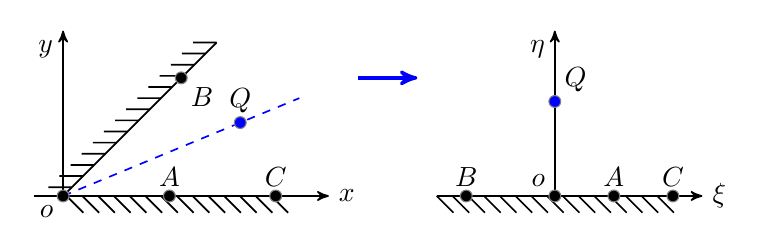
\begin{tikzpicture}[ media/.style={font={\footnotesize\sffamily}},
    interface/.style={
        postaction={draw,decorate,decoration={border,angle=-45,
                    amplitude=0.3cm,segment length=2mm}}},scale=1.5]
%\draw(0.7,-0.22) rectangle (6.7,1.425);
\clip(0.7,-0.22) rectangle (6.7,1.425);
\draw[semithick,interface](2.3,1.3)--(1,0)--(3,0);
\draw[semithick,->,>=stealth'](3,0)--(3.25,0) node[right]{$x$};
\draw[semithick,->,>=stealth'](0.75,0)--(1,0) (1,0)--(1,1.4) node[below left]{$y$};

\draw[semithick,dashed,blue](1,0)--(3,0.8284);

\fill[blue,draw=gray](2.5,0.6213) circle(0.05) node[above,black]{$Q$};

\fill[black,draw=gray](1,0)circle(0.05)node[below left]{$o$};
\fill[black,draw=gray](2,1) circle(0.05) node[below right,black]{$B$};
\fill[black,draw=gray](1.9,0) circle(0.05) node[above,black]{$A$};
\fill[black,draw=gray](2.8,0) circle(0.05) node[above,black]{$C$};
\draw[very thick,blue,->,>=stealth'](3.5,1)--(4,1);

\begin{scope}[xshift=90]
\draw[semithick,interface](1,0)--(3,0);
\draw[semithick,->,>=stealth'](3,0)--(3.25,0) node[right]{$\xi$};
\draw[semithick,->,>=stealth'](2,0)--(2,1.4) node[below left]{$\eta$};

\fill[black,draw=gray](2,0)circle(0.05)node[above left]{$o$};
\fill[blue,draw=gray](2,0.8) circle(0.05) node[above right,black]{$Q$};
\fill[black,draw=gray](2.5,0) circle(0.05) node[above,black]{$A$};
\fill[black,draw=gray](3,0) circle(0.05) node[above,black]{$C$};
\fill[black,draw=gray](1.25,0) circle(0.05) node[above,black]{$B$};
\end{scope}
\end{tikzpicture}

\vspace{-0.25em}
\caption{\label{p6f1}保角变换示意图}
\end{minipage}%
\begin{minipage}[b]{.35\textwidth}
\centering
\begin{tabular}{l|lll}
\multicolumn{1}{c|}{} & \multicolumn{1}{c}{$z$} & \multicolumn{1}{c}{$\alpha_i$} & \multicolumn{1}{c}{$a_i$} \\
\hline
\multicolumn{1}{c|}{A} & \multicolumn{1}{c}{1} & \multicolumn{1}{c}{$\pi$} & \multicolumn{1}{c}{1} \\
\multicolumn{1}{c|}{B} & \multicolumn{1}{c}{$\infty e^{i\alpha}$} & \multicolumn{1}{c}{$\pi$} & \multicolumn{1}{c}{$-\infty$} \\
\multicolumn{1}{c|}{C} & \multicolumn{1}{c}{$\infty$} & \multicolumn{1}{c}{$\pi$} & \multicolumn{1}{c}{$\infty$} \\
\multicolumn{1}{c|}{O} & \multicolumn{1}{c}{0} & \multicolumn{1}{c}{$\alpha$} & \multicolumn{1}{c}{0} \\
\end{tabular}
\caption{\label{p6f2}变换前后对应点的关系}
\end{minipage}
\end{figure}

\noindent 由Schwarz-christoffel变换
\begin{eqnarray}
\frac{dz}{d\zeta} &=& K\Pi_{i=1}^N(\zeta-a_i)^{\beta_i}, {~~} \beta_i = \frac{\alpha_i}{\pi}-1\nonumber\\
&=& K\zeta^{\alpha/\pi-1}\nonumber
\end{eqnarray}
积分可得$z=K\zeta^{\alpha/\pi}$或$\zeta=(z/K)^{\pi/\alpha}$,由$A,B,C,O$可得$K=1$, 代入$Q$点
\[
\zeta_0 = z_0^{\pi/\alpha} = a^{\pi/\alpha}e^{i\pi/2} = ia^{\pi/\alpha}
\]
又由镜像法可得$\xi-\eta$平面上的复速度势
\[
W(\zeta) = \frac{Q}{2\pi}\ln(\zeta-\zeta_0) + \frac{Q}{2\pi}\ln(\zeta-\overline{\zeta_0})
\]
因此$z$平面上的复速度势
\begin{eqnarray}
W(z) &=& \frac{Q}{2\pi}\ln(z^{\pi/\alpha}-ia^{\pi/\alpha}) + \frac{Q}{2\pi}\ln(z^{\pi/\alpha}+ia^{\pi/\alpha})\nonumber\\
&=&\frac{Q}{2\pi}\ln(z^{2\pi/\alpha} + a^{2\pi/\alpha})\nonumber
\end{eqnarray}
\end{solution} 
